%!TEX root = ../thesis.tex

% Definitions:
%%%%%%%%%%%%%%
% Semantiv Web = samantisches Web

\chapter{Grundlagen} % (fold)
\label{cha:grundlagen}

\todo[inline]{\Huge mehr QUELLEN!!!}
\todo[inline]{Grundlagen Einleitung schreiben}

\section{Zugriff auf Webanwendungen} % (fold)
\label{sec:zugriff_auf_webanwendungen}

Der Zugriff auf Daten von einer Webanwendung ist in den seltensten Fällen durch eine direkte Anbindung an die dahinter liegende Datenbank möglich beziehungsweise gewünscht. Gerade wenn das eigene Geschäft von diesen Daten abhängt, will man nur ungern alles mit allen teilen. Um trotzdem Dritten die Nutzung zu ermöglichen, wird dazu eine eine der Zugriff über eine vordefinierte Programmierschnittstelle (API) gestattet. Für Anwendungen und Dienste im Web sind die folgenden zwei Ansätze für die Architektur einer solchen API besonders verbreitet. 

\subsection{Representational State Transfer (REST)} % (fold)
\label{sub:rest}

Eine sehr beliebte Architektur für den öffentlichen Zugriff auf Webanwendungen ist \emph{Representational State Transfer} (REST) \cite[S.\,76]{fielding2000architectural}. REST baut auf HTTP auf und definiert einige Beschränkungen die eine REST basierter Dienst erfüllen muss. 

Die Grundidee besteht darin, dass hinter einer URL eine bestimmte Ressource sich verbirgt auf die man von außen zugreifen möchte. REST schreib aber nicht vor in welchen Datenformat diese Ressource übermittelt werden soll, sondern dass das zurückgelieferte Format der Ressource änderbar ist. 

\begin{quote}
\enquote{REST components communicate by transferring a representation of a resource
in a format matching one of an evolving set of standard data types, selected dynamically
based on the capabilities or desires of the recipient and the nature of the resource.}\cite[S.\,87]{fielding2000architectural} 

\end{quote}

Dadurch soll einer einfachere Verwendbarkeit in unterschiedliche Systemen ermöglicht werden. So kann für eine Webanwendung beim aufrufen im Browser eine HTML-Datei zurück geliefert werden, die sofort betrachtet werden kann und falls ein Programm darauf zugreift wird ein maschinenlesbares Format verwendet. Neben HTML sind auch noch XML und JSON sehr verbreitete Formate. Die Kommunikation wird dabei komplett Zustandslos abgehalten und alle Zusatzinformationen müssen immer mitgeliefert werden. Durch die Zustandslosigkeit skaliert das System viel besser, da Ressourcen sofort wieder frei gegeben werden können und nicht für spätere Anfragen gespeichert werden müssen. 

\begin{table}[ht]
\centering
\caption{Wichtigsten HTTP Operationen mit REST} 
\begin{tabular}{r|p{12cm}}
    \textbf{Operation} & 
    \textbf{Beschreibung} \\ 
    \hline
    \texttt{GET} & 
    Liefert die hinter einer URL liegende Ressource an den Aufrufer zurück.\\
    
    \texttt{POST} & 
    Dient zum Anlegen einer neuen Ressource. Die URI der neuen Ressource ist beim Aufruf noch unbekannt und wird von Service bestimmt. \\

    \texttt{PUT} & 
    Wird zum Ändern eine bestehenden Ressource genutzt. \\
    
    \texttt{DELETE} &
    löscht, wie der Name schon sagt, eine Ressource dauerhaft.
\end{tabular}
\label{tbl:rest_oprations}
\end{table} 

Wie schon beschrieben, nutzen REST basierte Dienste HTTP als Grundlage zur Kommunikation. Die dort definierten Operationen werden mit REST zur Auslieferung und Manipulation der Ressourcen verwendet. Zur Grundausstattung  gehören dabei \texttt{GET}, \texttt{POST}, \texttt{PUT} und \texttt{DELETE} (siehe Tabelle \ref{tbl:rest_oprations}). Die anderen Operationen \texttt{HEAD}, \texttt{TRACE}, \texttt{OPTIONS} und \texttt{CONNECT} sind eher selten anzutreffen.
     
% subsection rest (end)

\subsection{Simple Object Access Protocol (SOAP)} % (fold)
\label{sub:soap}

Das \emph{Simple Object Access Protocol}\cite{Mitra2007} (SOAP) ist ein vom W3C standardisiertes Netzwerkprotokoll für den Austausch von Daten zwischen heterogenen Systemen. SOAP schreibt einen bestimmten Aufbau von Nachrichten vor, innerhalb von denen die Daten transportiert werden. Als Repräsentation für diese Nachrichten wird auf XML gesetzt. Bei der Wahl des Transportprotokolls werden dahingegen keine Vorgaben gemacht und es ist frei wählbar. Häufig wird es aber in Verbindung mit HTTP und TCP verwendet. 


\begin{lstlisting}[
    language=XML,
    caption={SOAP Nachricht}\label{lst:soap_nachricht},
    captionpos=t]
<Envelope xmlns="http://www.w3.org/2003/05/soap-envelope">
    <Header>
        <!-- header information -->
    <Header> 
    <Body>
        <!--body content-->
    </Body>
</Envelope>
\end{lstlisting}

Eine Nachricht besteht im Grunde aus drei Elementen: den \emph{Envelope}, einen optionalen \emph{Header} und einem \emph{Body} (siehe Listing \ref{lst:soap_nachricht}). Der Envelope fungiert, wie die Übersetzung schon sagt, als Briefumschlag für die zu transportierenden Daten. Innerhalb jedes Envelopes können zusätzliche Meta-Informationen im Header Element gespeichert werden. Die eigentlichen Daten befinden sich im Body Element des Evelopes. Wie der Inhalt von Header und Body auszusehen haben wird von SOAP nicht vorgeschrieben. Dies können weitere XML Elemente oder einfache Zeichenketten sein. 

\subsubsection{Web Services Description Language} % (fold)
\label{ssub:wsdl}

% subsubsection wsdl (end)

Gebräuchlich ist der Einsatz von SOAP bei sogenannten \emph{Remote Procedure  Calls} (RPC). Unter RPC verseht man den Aufruf eine Funktion von einem entfernten Dienst und das Zurückliefern einer eventuell vorhandenen Antwort. Welche Funktionen von einen Dienst zur Verfügung stehen wird ein einer \emph{Web Services Description Language}\cite{wsdl2001} (WSDL) Datei beschrieben. Diese WSDL Datei wird in XML Format geschrieben und enthält alle wichtigen Informationen für RPC Aufrufe, die von einen Dienst zur Verfügung gestellt werden: 

\begin{description}
    \item[\textbf{types}] enthält Definition von Datentypen die in einer Message eingesetzt werden können. Zur Definition der Datentypen wird das Vokabular von XML Schema\footnote{\url{http://www.w3.org/XML/Schema}} eingesetzt.
    \item[\textbf{message}] Elemente beschreiben die Datentypen aus denen eine Nachricht aufgebaut ist.
    \item[\textbf{portType}] definiert eine Menge an zur Verfügung stehenden Operationen. Inklusive Eingabe- und Ausgabeparameter. In der WSDL Version 2.0 wurde portType in \emph{interface} umbenannt.
    \item[\textbf{binding}] beschreibt das Format und den Protokollablauf mehrerer Operationen. Zum Beispiel wie Eingabe- und Ausgabeparameter kodiert werden sollen. 
    \item[\textbf{port}] Definiert eine Adresse hinter der sich ein Binding befindet. Üblicherweise in Form ein URI. Seit WSDL 2.0 wird statt port der Begriff \emph{endpoint} verwendet.
    \item[\textbf{service}] dient zum Zusammenfassen mehrerer Ports zu einen einzigen Dienst.
\end{description}

Wird eine solche WSDL Datei öffentlich zugänglich gemacht, kann festgestellt werden welche Funktionen ein Dienst anbietet und automatisch APIs für unterschiedliche Systeme generiert werden. Der weiter Datenaustausch erfolgt dann über SOAP Nachrichten.

% subsection wsdl_und_soap (end)

% section zugriff_auf_webanwendungen (end)

\section{Datenintegration} % (fold)
\label{sec:datenintegration}

\todo[inline]{Datenintegration-Einleitung schreiben}

\subsection{Semantic Web} % (fold)
\label{sub:semantic_web}

Seit den Anfängen des \emph{World Wide Webs} (kurz als WWW oder Web bezeichnet) hat die Masse an abrufbaren Information immer mehr zugenommen. Die Vorteile des Webs liegen eindeutig in der guten Aktualität und Erreichbarkeit von überall auf Erde. Die Menge an Informationen sind aber auch ein Problem im Web. Da diese überall verteilt sind, ist es schwer für einen einzelnen alleine alles zu einem Thema zu finden. Suchmaschinen wie Google\footnote{\url{https://www.google.com}}, Yahoo\footnote{\url{yahoo.com}} oder Microsoft Bing\footnote{\url{http://www.bing.com/}} leisten hier gute Dienste. Doch für Maschinen ist es noch immer nicht einfach die Inhalte von Webseiten zu verstehen, da diese für Menschen gemacht wurden \cite{Hitzler2008a}. Auch der erlernen von neuen Wissen anhand vorhandener Informationen ist in der aktuellen Form des Webs nur schwer realisierbar. 

2001 machte Tim Berners-Lee (der Erfinder des Webs) den Vorschlag \cite{Berners-Lee2001} das Web mit maschinenlesbaren Informationen zu erweitern und so die Verarbeitung mit Computerprogrammen zu vereinfachen. Die Idee des \emph{Semantic Webs} wurde geboren. Der Inhalt des Webs wird mit semantischen Information so erweitert, dass Programme das sich zwei Texte an unterschiedlichen Stellen des Webs um das selbe Thema handeln. Aber auch die Anzeige von impliziten Wissen, wenn jemand zum Beispiel eine Telefonnummer in Los Angeles, USA sucht und aus Deutschland anrufen will, wird im mitgeteilt dass er wegen der Zeitdifferenz von neun Stunden lieber erst Nachmittags anrufen sollte, wäre so einfacher möglich.

\subsubsection{Resource Description Framework} % (fold)
\label{ssub:resource_description_framework}

Eine Baustein des Semantic Webs ist das \emph{Resource Description Framework} (RDF). Wie der Name schon suggeriert, dient RDF zur Beschreibung von einzelnen Ressourcen innerhalb des Webs. Nach \cite{Klyne2004,Manola2004} bestand die Motivation bei der Entwicklung von RDF Information über Ressource in einen offenen Datenmodell zu speichern, so dass diese Daten von Maschinen automatisch verarbeitet, manipulieren und untereinander ausgetauscht werden können. Gleichzeitig sollte es auch einfach von jedem erweitert werden können \enquote{RDF is designed to represent information in a minimally constraining, flexible way}\cite{Klyne2004}.

Das Datenmodell von RDF ist zur effizienten Verarbeitung sehr einfach aufgebaut. Die Grundlage bilden Tripel aus Subjekt, Prädikat und Objekt. Einer oder mehrere solcher Triple zusammen werden als gerichteter RDF-Graph bezeichnet. Subjekt und Objekt stehen über das Prädikat mit einander in Beziehung, wobei die Beziehung immer vom Subjekt zum Objekt geht. Das Prädikat wird auch als Eigenschaft (engl. Property) bezeichnet. Gemeinsam beschreibt das Triple immer eine Aussage über eine oder zwei Ressourcen. Zum Beispiel \enquote{Die Dose enthält Kekse} wäre eine Aussage, dass in einer Dose sich Kekse befinden. Die Dose ist dabei das Subjekt, enthält das Prädikat und Kekse das Objekt. Ein Triple ist quasi ein einfacher Satz in der natürlichen Sprache \cite{Heinzen}. Für Subjekt, Prädikat und Objekt werden in RDF \emph{Uniform Resource Identifier} (URI), \emph{Literale} oder \emph{leere Knoten} (im englischen \emph{Blank Nodes} genannt) verwendet. 

\begin{description}
    \item[URIs] sind eindeutige Bezeichner die eine beliebige reale oder abstrakte Ressource darstellen und werden wie in RFC 2396\footnote{\url{http://www.isi.edu/in-notes/rfc2396.txt}} beschrieben formatiert. Relative URIs sollten aber nach \cite{Klyne2004} aber nach Möglichkeit vermieden werden. URIs bilden eine Verallgemeinerung der im Web gebräuchlichen Uniform Resource Locator (URL).
   
    \item[Literale] bestehen aus einfachen Zeichenketten die zum Speichern der Informationen dienen. Zusätzlich können Literale mit der Angabe der verwendeten Sprache \texttt{"Objekt"@de} oder des Datentyps \texttt{"42"^^xsd:integer} erweitert werden. Bei Literalen ist darauf zu achten, dass die Literale \texttt{"Objekt"} und \texttt{"Objekt"@de} auf den ersten Blick zwar den selben Wert beschreiben, aber aus Sicht von RDF nicht die selben sind. Sowohl die angegebene Spracht als auch der Datentyp müssen übereinstimmen.

    \item[Leere Knoten] werden als alle Knoten im RDF Graphen beschrieben, welche weder eine URI noch ein Literal sind. Sie dienen häufig dazu, um Subjekte zu beschreiben für die nicht unbedingt eine eigene URI nötig ist und sind nur innerhalb eines Graphen eindeutig. Für die Referenzierung außerhalb des RDF-Graphen sind leere Knoten ungeeignet.
\end{description}

Doch nicht jeder davon ist in jeden Teil des Tripels erlaubt. Das Subjekt ist entweder eine URI oder ein leerer Knoten, wobei das Prädikat nur eine URI sein kann. Dahingegen ist es beim Objekt möglich eine URI, einen leeren Knoten oder ein Literal zu verwendeten. 

% subsubsection resource_description_framework (end)

\subsubsection{Darstellung von RDF-Graphen} % (fold)
\label{ssub:darstellung_von_rdf_graphen}

In Laufe der Zeit von RDF wurde verschiedene Möglichkeiten erfunden einen RDF-Graphen darzustellen. In diesem Abschnitt werden drei Formen vorgestellt die auch in dieser Arbeit zur Visualisierung benutzt werden. 

\paragraph{Graphische Darstellung} % (fold)
\label{par:graphische_darstellung}

Graphisch lässt sich RDF als gerichteter Graph mit Knoten und Kanten darstellen. Ressourcen werden dabei als elliptische Knoten, Literale als Rechtecke und die Prädikate als gerichtete Kante gezeichnet. Ein Beispiel ist in Abbildung \ref{fig:graphisch_rdf_triple} zu sehen.

    \begin{figure}[ht]
        \centering
        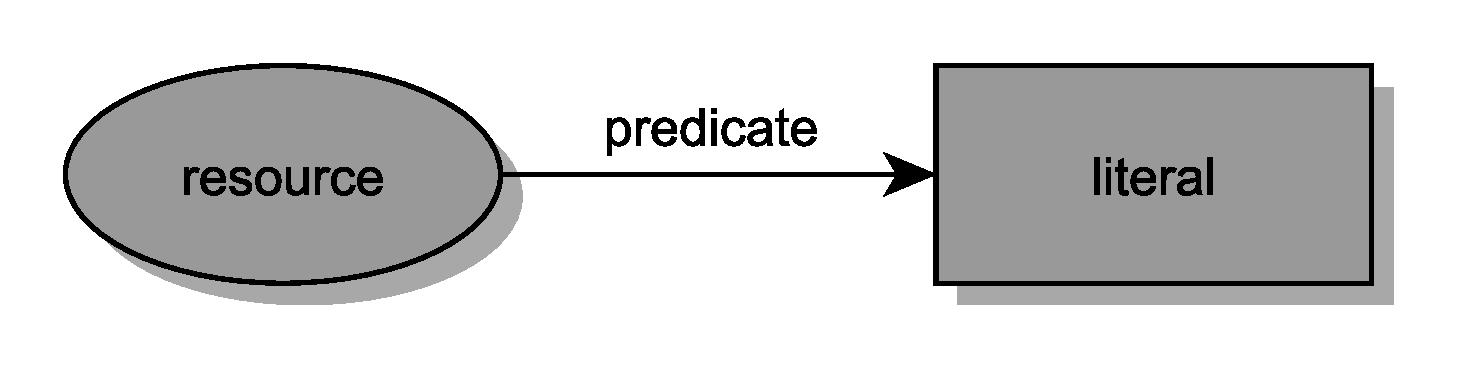
\includegraphics[
            width=0.6\textwidth,
            keepaspectratio=true,
            clip=true]
            {assets/images/rdf-triple}
        \caption{Einfacher RDF-Graph}
        \label{fig:graphisch_rdf_triple}
    \end{figure}

% paragraph graphische_darstellung (end)

\paragraph{RDF/XML} % (fold)
\label{par:rdf_xml}

RDF/XML\cite[Abschnitt 3.2]{Manola2004} ist eine verbreitete Form RDF-Dokumente zu beschreiben. Die Basis bildet hierbei die Verwendung der Extensible Markup Language (XML). In Listing \ref{lst:rdf_xml_beispiel} ist ein Beispieldokument in RDF/XML zusehen. Das in Zeile 2 zu sehende \texttt{rdf:RDF} Element zeigt, dass sich innerhalb von ihm sich die RDF-Beschreibung des Dokuments befindet. In diesem ELement werden mit \texttt{xmlns:} einige Präfixe für Namensräume  definiert, um das Dokument übersichtlicher zu halten. Alle Präfixe werden danach mit den angegebenen Namensraum ersetzt. Das \texttt{Description} in Zeile 5 stellt die Beschreibung einer Ressource im RDF-Graphen. Die URI der Ressource wird mit dem Attribut \texttt{rdf:about} definiert. Innerhalb des Description Elements befinden sich die Prädikate. In Zeile 6 steht also, dass die Ressource die Eigenschaft \texttt{exterms:enthaelt} besitzt und diese das Literal \texttt{Kekse}. Wäre das Objekt nicht wie hier ein Literal sondern eine weitere Ressource, könnte man über das Attribut \texttt{rdf:ressource} für das \texttt{exterms:enthaelt} auf diese Ressource verweisen.

\begin{lstlisting}[
    language=XML,
    caption={RDF/XML Beispiel}\label{lst:rdf_xml_beispiel},
    captionpos=t]
<?xml version="1.0"?>
<rdf:RDF xmlns:rdf="http://www.w3.org/1999/02/22-rdf-syntax-ns#"
    xmlns:exterms="http://www.example.org/terms#">

    <rdf:Description rdf:about="http://www.example.org/dose">
       <exterms:enthaelt>Kekse</exterms:enthaelt>
    </rdf:Description>
</rdf:RDF>
\end{lstlisting}
% paragraph rdf_xml (end)

\paragraph{Turtle} % (fold)
\label{par:turtle}

Turtle (Ausgeschrieben: \emph{Terse RDF Triple Language}) ist eine weiter Möglichkeit RDF-Graphen darzustellen und ist eine ging aus der Sprache N3 (Kurzform für Notation 2) hervor \cite{DavidBeckett}. In Turtle wird das Triple aus Subjekt, Prädikat und Objekt hintereinander geschrieben und zwischen jeden mindestens ein Leerzeichen gelassen. Als Abschluss folgt nach jedem Tripel noch ein Punkt. Der Punkt verdeutlicht noch einmal die Ähnlichkeit mit gesprochenen Sätzen. Listing \ref{lst:turtle_beispiel} zeigt das Beispiel mit der Keksdose noch einmal in Turtle Notation. 

\begin{lstlisting}[
    caption={Turtle Beispiel}\label{lst:turtle_beispiel},
    captionpos=t]
<http://www.example.org/dose> <http://www.example.org/terms#enthaelt> "Kekse" .
\end{lstlisting} 

In Turtle ist darauf zu achten, dass alle URIs immer zwischen Spitzenklammern stehen müssen. Literale werden in Anführungszeichen geschrieben. Da nun einzelne Prädikate beziehungsweise allgemein URIs recht häufig innerhalb eines Graphen auftauchen können, kann es einfacher sein diese abzukürzen. Wie schon in RDF/XML können auch in Turtle Präfixe definiert werden um Schreibarbeit zu sparen.

\begin{lstlisting}[
    caption={Turtle Präfixe}\label{lst:turtle_prefix},
    captionpos=t]
@prefix exterms: <http://www.example.org/terms#> .
<http://www.example.org/dose> exterms:enthaelt "Kekse" .   
\end{lstlisting}

In der ersten Zeile von Listing \ref{lst:turtle_prefix} wird durch Einleiten mit dem Schlüsselwort \texttt{@prefix} ein neuer Präfix \texttt{exterms:} für den Namensraum \texttt{http://www.example.org/terms\#} festgelegt. Dieser Präfix kann nun überall innerhalb des Dokumentes verwendet werden, wobei die Spitzenklammern dann weggelassen werden können.

\begin{lstlisting}[
    caption={Turtle abkürzende Schreibweise}\label{lst:turtle_shortcut},
    captionpos=t]
@prefix exterms: <http://www.example.org/terms#> .
<http://www.example.org/dose> exterms:farbe "blau";
    exterms:enthaelt "Kekse", "Geld" .   
\end{lstlisting}

Listing \ref{lst:turtle_shortcut} zeigt nochmal ein drittes Beispiel, wie redundante Angeben eingespart werden. Wie man in der zweiten Zeile sehen kann. wir deine Frage für die Dose angeben das Triple aber mit einen Semikolon abschlossen und nicht mit einen Punk. Durch das Semikolon ist es Möglich das Subjekt mehrfach wieder zu verwenden, wenn sich nur Prädikat und Objekt ändern. So können sich mehrere Eigenschaften einer Ressource platzsparend schreiben ohne das Subjekt immer wieder anzugeben. Ändert sich dahingegen nur das Objekt können mehrere durch Kommata getrennt hintereinander geschrieben werden. Die dritte Zeile beschreibt zum Beispiel, dass in der Dose nicht nur Kekse sonder auch Geld steckt. Leere Knoten können dann noch in Turtle durch angeben einer geöffneten eckigen Klammer gefolgt von einer sich Schließenden dargestellt \enquote{\texttt{[]}}. Soll ein leerer Knoten innerhalb eines Graphen referenziert werden, kann er auch als \texttt{\_:LABEL}, wobei \texttt{LABEL} ein beliebiger Beizeichner ist, geschrieben werden.

% paragraph turtle (end)

% subsubsection darstellung_von_rdf (end)

\subsubsection{Ontologien} % (fold)
\label{ssub:ontologien}

Sollen Daten aus verschiedenen Quellen zusammengefügt werden, stellt sich häufig das Problem dass Teile dieser dieser Daten zwar den gleichen Sinn haben, aber aufgrund der Sichtweise des jeweiligen System eine andere Bezeichnung besitzen. Das kann zum Beispiel zu Missverständnissen bei der Verarbeitung führen oder dass Teile eines anderen Systems nicht wiederverwendet werden können \cite{Uschold1996a}. Einen Ausweg aus diesem Dilemma kann die Verwendung von Ontologien zeigen. Ontolgien können allgemein als Wissensbasis \cite{Uschold1996a,Hitzler2008a} bezeichnet werden und liefern eine formale Spezifikation über eine bestimmte Interessensdömäne. Sie beschreibt nicht nur wie das verwendete Vokabular aussieht, sondern legt auch fest welche einheitliche Bedeutung jede Vokabel hat. 

Im Bereich des Semantic Webs sind heutzutage zwei Sprachen für die Erstellung von Ontologien weit verbreitet. Diese sind \emph{RDF Schema} (RDFS)\cite{Brickley} und die darauf aufbauende \emph{Web Ontology Language} (OWL)\cite{partelschneider2004}. Beide Sprachen basieren auf RDF, so können sie zusammen mit jedem System verwendet werden, das RDF versteht. Mit ihnen ist man im Stande Klassen von abstrakten Objekten und deren Eigenschaften zu definieren und diese in eine Vererbungshierarchie einzugliedern. Im Gegensatz zu RDFS können in OWL diverse Einschränkungen definiert werden, wie zum Beispiel dass eine Eigenschaft nur einmal pro Objekt einer Klasse vorhanden sein darf. Die Anhänge \ref{sec:socc_connector_config_ontologie} und \ref{sec:sioc_services_authentication_module} zeigen zwei Ontologien in der Sprache OWL, welche innerhalb dieser Arbeit entwickelt wurden und in Abschnitt \ref{sub:connector_config_ontologie} und \ref{sub:autorisierung_und_authentifizierung} beschreiben werden.

% subsubsection ontologien (end)

% subsection semantic_web_und_das_resource_description_framework (end)

\subsection{Friend of a Friend (FOAF)} % (fold)
\label{sub:friend_of_a_friend_}

\emph{Friend of a Friend}\footnote{\url{http://www.foaf-project.org}} (FOAF) ist ein 2000 gestartet Projekt und versucht Personen innerhalb des Webs, inklusive der Verbindungen zwischen ihnen und anderen, sowie dem was sie machen, in maschinenlesbarer Form abzubilden. FOAF stellt hierzu ein Vokabular \cite{Brickley2010} auf der Basis von RDF für solche sozialen Netzwerke zur Verfügung. Das Vokabular von FOAF gliedert sich dazu in einen \enquote{FOAF Core} und einen \enquote{Social Web} Bereich. Der Core-Bereich die Klasse \texttt{Agent} für alle Dinge die eine Handlung ausführen können, also sowohl natürliche Personen, Gruppen oder Organisationen als auch Computerprogramme oder Maschinen. Für diese gibt es jeweils noch einzelne Unterklassen die von der Klasse \texttt{Agent} erben. Objekten dieser Klassen können eigene Eigenschaften wie einen Namen, ein Alter oder wen sie kennen gegeben werden. Der Sozial Web Bereich enthält alle Teile die für das Web interessant wären. Das wären zum Beispiel welche E-Mail-Adresse eine Person besitzt, welche Benutzerkonten im bei welcher Webseite gehören oder wie die URL seiner Homepage lautet. Das FOAF Projekt sieht sich aber selber nicht als Konkurrenz gegenüber den etablierten sozialen Online-Netzwerken, sondern eher ein Ansatz für einen besser Austausch zwischen den einzelnen Seiten \cite[Abstract]{Brickley2010}.

Listing \ref{lst:foaf_beispiel} zeig eine Beispiel FOAF-Dokument in RDF/XML. Es beschreibt die fiktive Person \enquote{Max Mustermann}, mit Vor- und Nachname sowie der Hashwert seiner E-Email-Adresse (\texttt{foaf:mbox\_sha1sum}). Diese Person kennt (\texttt{foaf:knows}) kennt eine Person mit dem Namen \enquote{John Doe} der ebenso eine E-Mail-Adresse mit den angegeben Hashwert besitzt. Statt die Eigenschaften von John Doe hier noch einmal vollständig anzugeben, wird über die Eigenschaft \texttt{rdfs:seeAlso} auf ein weiteres FOAF-Dokument verwiesen, dass die fehlenden Daten enthält. 

\begin{lstlisting}[
    language=XML,
    caption={FOAF Beispiel}\label{lst:foaf_beispiel},
    captionpos=t]
<rdf:RDF xmlns:rdf="http://www.w3.org/1999/02/22-rdf-syntax-ns#"
         xmlns:rdfs="http://www.w3.org/2000/01/rdf-schema#"
         xmlns:foaf="http://xmlns.com/foaf/0.1/">
  <foaf:Person>
    <foaf:name>Max Mustermann</foaf:name>
    <foaf:firstName>Max</foaf:firstName>
    <foaf:surname>Mustermann</foaf:surname>
    <foaf:mbox_sha1sum>dce4fc922158f8b26fbf0a65ea32bfab58488bd2</foaf:mbox_sha1sum>
    <foaf:knows>
      <foaf:Person>
        <foaf:name>John Doe</foaf:name>
        <foaf:mbox_sha1sum>479ea35d3522662b70dc7afd721853485c95db57</foaf:mbox_sha1sum>
        <rdfs:seeAlso rdf:resource="http://www.example.org/people/jd/foaf.rdf"/>
      </foaf:Person>
    </foaf:knows>
  </foaf:Person>
</rdf:RDF>
\end{lstlisting}

% subsection friend_of_a_friend_ (end)

\subsection{Semantically-Interlinked Online Communities (SIOC)} % (fold)
\label{sub:semantically_interlinked_online_communities}

\emph{Semantically-Interlinked Online Communities} (SIOC, ausgesprochen \enquote{schock}) ist ein Projekt, welches von Uldis Boj\=ars und John Breslin begonnen wurde um unterschiedliche, webbasierte Diskussionslattformen(Blog, Forum, Mailinglist,\dots) untereinander verbinden zu können \cite{deri2013,Breslin2005,Bojars2008a}. Der Kern von SIOC besteht aus einer Ontologie, welche den Inhalt und die Struktur diese Plattformen in ein maschinenlesbares Format bringt und es erlaubt diese auf semantischer Ebene zu verbinden. Auch soll es so möglich sein Daten von einer Plattform zu einer Anderen zu transferieren und so einfacher Inhalte austauschen zu können. Als Basis für SIOC dient RDF, die Ontologie selber wurde in RDFS und OWL designt. Um nicht das Rad neu erfinden zu müssen greift SIOC auf schon bestehende und bewährte Ontologien zurück. Für die Abbildung von Beziehungen zwischen einzelnen Personen wird FOAF und für einige Inhaltliche- und Metadaten (Titel, Inhalt, Erstelldatum, \dots) Dublin Core Terms\footnote{\url{http://dublincore.org/documents/dcmi-terms}} eingesetzt.

\begin{figure}[ht]
    \centering
    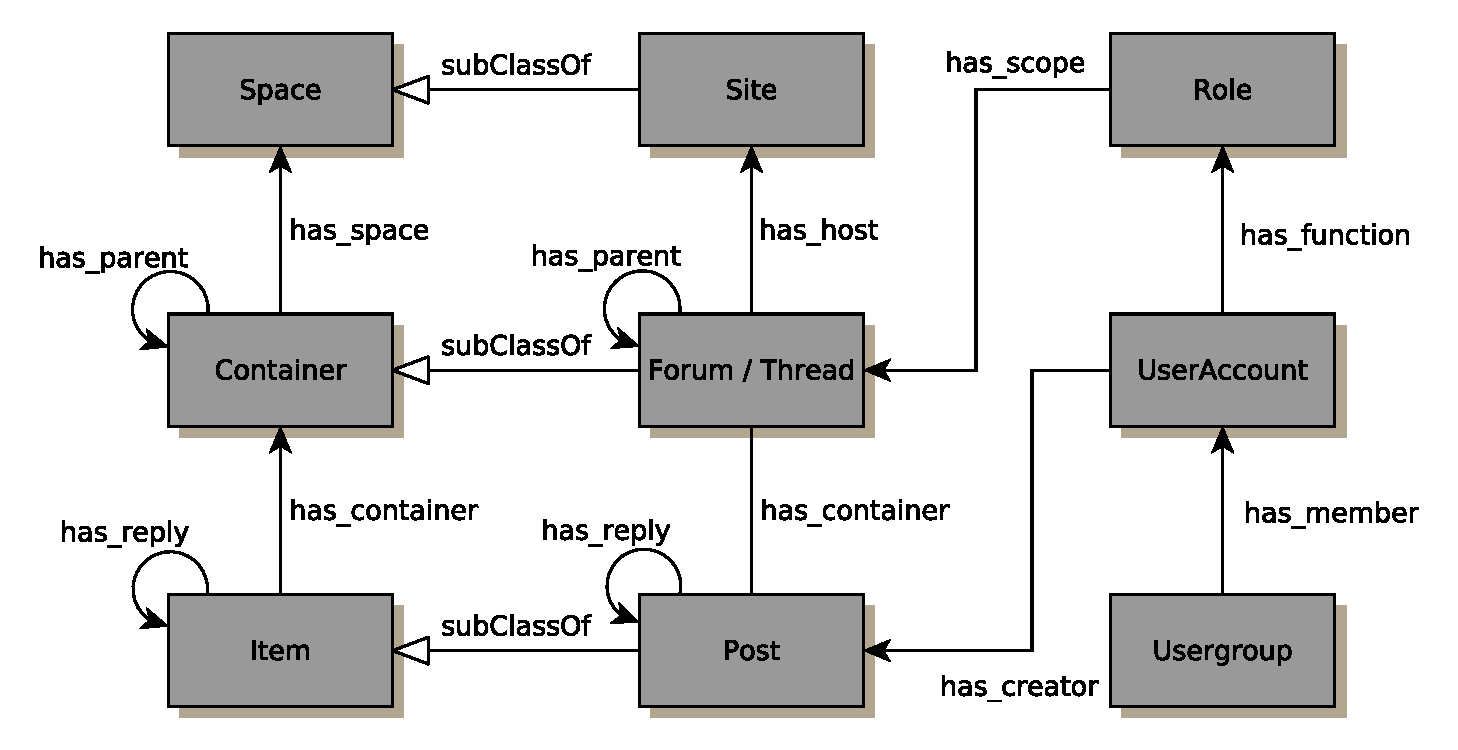
\includegraphics[
        width=\textwidth,
        keepaspectratio=true,
        clip=true]
        {assets/images/sioc_overview}
    \caption{Aufbau von SIOC (modifiziert) - Originalquelle: \cite{deri2013}}
    \label{fig:sioc_aufbau_diagramm}
\end{figure}

Die wichtigsten Klassen von SIOC sind in Abbildung \ref{fig:sioc_aufbau_diagramm} in der mittleren Spalte zu sehen. Die Klasse \texttt{Site} ist für die Beschreibung von allgemeinen Webseiten in denen Beiträge innerhalb von Containern verfasst werden. Ein solcher Container ist die Klasse \texttt{Forum}und steht für einen Ort an dem Diskussionen geführt werden. Enthält ein Forum unterschiedliche Diskussionen zu unterschiedlichen Themen, kann es noch einmal in unterschiedliche \texttt{Thread} unterteilt werden, welche immer ein Forum als Elternteil haben (\texttt{has\_parent}). Beide Klassen leiten sich von der Klasse \texttt{Container} als einen allgemeinen Ort für Beiträge ab. Die einzelnen Beiträge werden durch die Klasse \texttt{Post} beziehungsweise von der übergeordneten Klasse \texttt{Item} modelliert. Beiträge gehören in der Regel immer zu einen bestimmten Container oder mindesten zu einer Webseite. Es ist auch mögliche Beiträge als Kommentar zu anderen Beiträgen über die Eigenschaft \texttt{has\_reply} abzubilden. Jeder Beitrag besitzt mindesten einen Autor der ein Benutzerkonto auf der betreffenden Seite besitzt. Für die Beschreibung eines solchen Benutzerkontos wird die Klasse \texttt{UserAccount} verwendet. Dieses Benutzerkonto kann nun zu einer Gruppe von anderen Konten gehören, zum Beispiel einer Lerngruppe. Über die Klasse \texttt{Role} keine einen Benutzerkonto eine bestimmte Rolle innerhalb eine Seite, Forum und so weiter zugeteilt werden. Ein Beispiel dafür wäre die Rolle eines Moderator, der überwacht ob die Regel der Seite in den einzelnen Foren eingehalten werden.

% subsection semantically_interlinked_online_communities (end)

% section datenintegration (end)

\section{Datenverteilung} % (fold)
\label{sec:datenverteilung}

\todo[inline]{Datenverteilung-Einleitung schreiben}

\subsection{Java Messaging Service} % (fold)
\label{sub:java_messaging_service}

Das \emph{Java Messageing Service} (JMS) ist ein Sammlung von Schnittstellen für das Erstellen, Senden und Empfangen von Nachrichten zwischen Clients \cite{jms}. JMS erlaubt eine Entwicklung von verteilten Anwendung die nicht nur lose gekoppelt, sondern auch asynchron und zuverlässig arbeiten. 

\begin{figure}[ht]
    \centering
    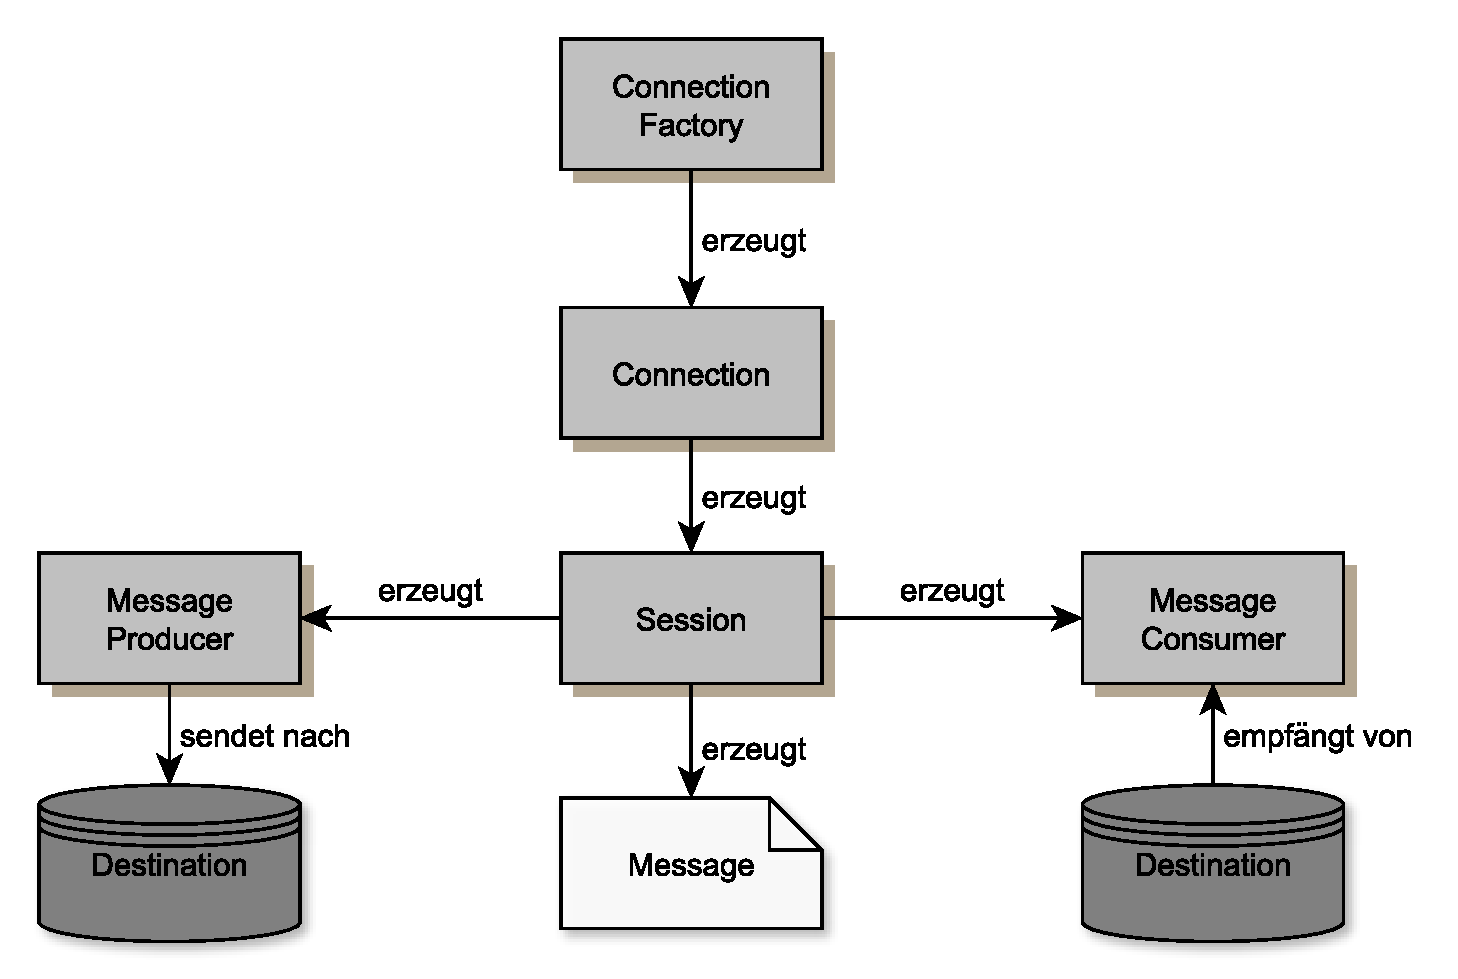
\includegraphics[
        width=0.8\textwidth,
        keepaspectratio=true,
        clip=true]
        {assets/images/jms_api_overview}
    \caption{JMS Programmiermodell - Original Bild: \url{http://docs.oracle.com/javaee/1.3/jms/tutorial/1_3_1-fcs/doc/images/Fig3.1.gif} (Zugriff: 2013-09-15)}
    \label{fig:jms_api_overview}
\end{figure}

Die Grundstruktur einer JMS Anwendung besteht aus einem \emph{JMS Provider}, der die Schnittstellen von JMS implementiert. Dieser JMS Provider wird auch all  \emph{Message Oriented Middleware} (MOM) bezeichnet und kümmert sich auch darum, dass Nachrichten zuverlässig verschickt werden. Einen JMS Client von dem Nachrich
ten verschickt und empfangen werden. Den Nachrichten selber und den sogenannten \emph{Administered Objects}. Diese bestehen aus vorkonfigurierten \emph{Connection Factory}s für das Erstellen von Verbindungen (Connections) zwischen Client und MOM und \emph{Destination}s als Sende- und Empfangspunkte von Nachrichten. Die Administered Objects können im Client über das Java Naming and Directory Interface (JNDI)\footnote{JNDI API:\url{http://www.oracle.com/technetwork/java/index-jsp-137536.html}} API abgefragt werden. Alle Clients die nicht die JMS API sondern die implementierte API der MOM direkt verwenden, werden \emph{Native Client} genannt.

JMS unterstützt zwei Verbindungsarten zum Übertragen von Nachrichten: Queue-basiert und Topic-basiert. Als Queue-basiert wird eine Punkt-zu-Punkt Verbindung bezeichnet. Hier werden Nachrichten nur zwischen zwei Clients übertragen und gegebenenfalls in einer Warteschlange zwischengespeichert. Hinter Topic-basiert verbirgt sich ein Publish-Subscribe Mechanismus bei dem ein Client Nachrichten an eine bestimmtes Topic-Destination schickt und andere Clients sich auf dieses Topic anmelden können, die dann die Nachrichten des ersten Clients zugeschickt bekommen. Ob Queue oder Topic-basiert, wird über das verwendete Destination Objekt ausgewählt.

Sollen nun Nachrichten von einem Client verschickt beziehungsweise empfangen werden, muss mit einer Connection Factory eine neue Connection zu einer MOM aufgebaut werden. Mit dieser Connection wird danach ein \emph{Session}-Objekt erstellt, das als Kontext zum Senden und Empfangen verwendet wird. Sollen Nachrichten gesendet werden, muss mit einem Destination-Objekt ein \emph{MessageProducer} und danach eine Nachricht mit dem Session-Objekt erstellt werden. Die Nachricht wird dann über den MessageProducer versendet. Für das Empfangen ist ein \emph{MessageConsumer} verantwortlich. Abbildung \ref{fig:jms_api_overview} zeig noch einmal den Zusammenhang aller JMS Komponenten.

\begin{lstlisting}[
    caption={JMS Beispiel}\label{lst:jms_beispiel},
    captionpos=t]
Context ctx = new InitialContext();
ConnectionFactory connectionFactory = (ConnectionFactory) ctx.lookup("ConnectionFactory");

Connection connection = connectionFactory.createConnection();
connection.start();

Session session = connection.createSession();
Destination destination = session.createTopic("topic-test");

MessageProducer msgProducer = session.createProducer(destination);
Message msg = session.createTextMessage("Hallo World!");
msgProducer.send(msg);
\end{lstlisting}

Listing \ref{lst:jms_beispiel} zeig ein kleines Beispiel zum Senden eine Textnachricht mit JMS. Die erste und zweite Zeile zeigt wie ein JNDI Kontext erstellt und nach einer vordefinierten Connection Factory mit den Name \enquote{ConnectionFactory} gesucht wird. Mit dieser Connection Factory wird dann eine neue Connection erstellt und gestartet. Danach folgt in Zeile 7 und 8 das Erstellen einer neuen Session und die Definition eins Topics mit dem Namen \enquote{topic-test} als Destination. In der zehnten Zeile wird dann der MessageProducer zum Senden von Nachrichten und in der Folgezeile die zu sendende Textnachricht erzeugt. Diese wird dann in der letzten Zeile an das Topic verschickt.

% subsection java_messaging_service (end)

\subsection{Enterprise Integration Pattern (EIP)} % (fold)
\label{sub:enterprise_integration_pattern}

Bezeichnungen wie \enquote{Iterator}, \enquote{Factory Method}, \enquote{Observer} oder \enquote{Proxy} hat bestimmt schon jeder Programmieren mindestens einmal gehört. Hierbei handelt es sich im sogenannte Entwurfsmuster für Softwareprogramme. Sie sind Schablonen für Lösungen von Problemen, die in der Entwicklung von Software immer wieder auftreten und sich als hilfreich erwiesen haben. Auch in der Integration von verschiedenen Geschäftsanwendungen in ein System treten solche Muster immer wieder auf. Gregor Hohpe und Bobby Woolf beschreiben in ihren Buch \enquote{Enterprise Integration Patterns: Designing, Building, and Deploying Messaging Solutions}\cite{Hohpe:2003:EIP:940308} eine Vielzahl solcher Enterprise Integration Patterns (EIP) für die Integration mit MOM. Alle hier aufzuzählen würde den Rahmen dieser Arbeit sprengen. Aus diesem Grund werden in Tabelle \ref{tbl:eip_beispiel_muster} fünf Muster inklusive der verwendeten Symbole vorgestellt die später noch vorkommen werden. Die restlichen Muster sind auf der Webseite von EIP\footnote{\url{http://www.enterpriseintegrationpatterns.com/toc.html}} zu finden.

\begin{table}[ht]
    \centering
    \caption{Einige Beispiel von EIP}
    \begin{tabular}{c|c|p{9cm}}
        \textbf{Icon} & 
        \textbf{Name} & 
        \textbf{Beschreibung} \\ 
        \hline

        \raisebox{-0.7\totalheight}{
\includegraphics[
            width=1cm,
            keepaspectratio=true]
        {assets/images/eip/message_alt}} & 
        \emph{Message} & 
        Über Nachrichten werden Daten zwischen zwei oder mehr Systemen ausgetauscht. \\

        \raisebox{-0.7\totalheight}{
\includegraphics[
                width=3cm,
                keepaspectratio=true]
            {assets/images/eip/channel}}& 
        \emph{Channel} &
        Ein Channel beschreibt einen Nachrichtenkanal über dem Nachrichten von einem Systemen in ein anderes verschickt werden können.\\

        \raisebox{-0.7\totalheight}{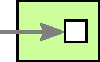
\includegraphics[
                width=3cm,
                keepaspectratio=true]
            {assets/images/eip/endpoint}}& 
        \emph{Endpoint} & 
        Endpoints sind Schnittstellen in einem System, von dem Nachrichten in einen Kanal gesendet oder von da Empfangen werden. \\
        &&\\


        \raisebox{-0.7\totalheight}{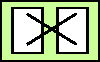
\includegraphics[
                width=3cm,
                keepaspectratio=true]
            {assets/images/eip/message_translator}} & 
        \emph{Message Translator} & 
        Nicht immer liegt eine Nachricht im richtigen Format für ein System vor. Durch Message Translators können diese in das gewünschte Format übersetzt werden.\\

        \raisebox{-0.7\totalheight}{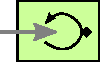
\includegraphics[
                width=3cm,
                keepaspectratio=true]
            {assets/images/eip/polling_consumer}}& 
        \emph{Polling Consumer} &

    \end{tabular}
    \label{tbl:eip_beispiel_muster}
\end{table}

\subsubsection{Apache Camel} % (fold)
\label{ssub:apache_camel}

\emph{Apache Camel}\cite{ApacheCamel} (kurz: Camel) ist ein Projekt der Apache Software Foundation (kurz: Apache) für das Routen und Verteilen von Nachrichten zur Integration von System auf der Basis von definierten Regeln. Camel stellt dazu eine Java basierte API für den Einsatz der EIP bereit. Die Regeln für die Routen, die Nachrichten nehmen können, können direkt in Java aber auch durch das Spring Framework\footnote{\url{http://www.springsource.org/}} in XML definiert werden. 

\begin{lstlisting}[
    caption={Apache Camel Beispiel}\label{lst:camel_beispiel},
    captionpos=t]
RouteDefinition rd = new RouteDefinition()
    .from('timer://helloTimer?period=3000')
    .to('log:helloLog');

CamelContext camelContext = new DefaultCamelContext();
camelContext.addRouteDefinition( rd );
camelContext.start();
\end{lstlisting}

Listing \ref{lst:camel_beispiel} zeig ein kleines Beispiel, wie eine Nachrichtenroute in Java definiert werden kann. In der ersten Zeile wird über die Klasse \texttt{RouteDefinition} eine neue Route erstellt. Über die Methode \texttt{from} wird der Endpunkt vom dem die Route ausgeht festgelegt. Welcher Endpunkt das genau seien soll kann auf zwei Arten definiert werden. Man übergibt der Methode direkt ein Objekt einer Klasse die das Interface \texttt{Endpoint} implementiert oder man macht es, wie hier im Beispiel, über eine URI. Die URI baut sich auf folgende Weise zusammen. Der Teil bis zum Doppelpunkt, das sogenannte \enquote{Schema}, legt die Komponente (engl. \texttt{Component}) fest, von der ein Endpunkt erzeugen werden soll. In diesem Falls ist es eine Timer-Komponente, deren Endpunkt im periodischen Abstand Event-Nachrichten verschickt. Der Rest der URI wird zur Konfiguration an den Endpunkt übergeben. \enquote{helloTimer} steht hier für einen Namen für den Timer und der Parameter \enquote{period} gibt den zeitlichen Abstand zwischen zwei Event-Nachrichten an. Das Ziel der Route wird mit der Methode \texttt{to} in Zeile Drei festgelegt. Für das Ziel wird hier eine Log-Komponente mit dem Namen \enquote{helloLog} festgelegt, die alle reinkommenden Nachrichten protokolliert. In der fünften Zeile wird ein \texttt{CamelContext} Objekt, das für die Verwaltung und Ausführung der Routen verantwortliche ist. Die eben erstellte Route wird dann dem CamelContext hinzugefügt und die Ausführung in der letzten Zeile gestartet. Nun Wird der Timer alle 3000 Millisekunden eine neue Event-Nachricht erzeugen und an den CamelContext schicken. Dieser leitet die Nachricht dann an das durch die Route definierte Ziel und wird dort von der Log-Komponente

% subsubsection apache_camel (end)

% subsection enterprise_integration_patternl (end)

% section datenverteilung (end)

\section{Lernplattformen und soziale Online-Netzwerke} % (fold)
\label{sec:lernplattformen_und_soziale_online_netzwerke}

An dieser Stelle sollen noch kurz einige Lernplattformen und soziale Online-Netzwerke vorgestellt, die im späteren Verlauf dieser Arbeit für die Implementierung verwendet wurden. Im Einzelnen waren dies \emph{Moodle}, \emph{Canvas}, \emph{Youtube}, \emph{Facebook} und \emph{Google+}, da sie einen guten Schnitt von den Plattformen bilden, die heutzutage sowohl im Bereich E-Learning als auch von der breiten Masse verwendet werden.

\subsection{Moodle} % (fold)
\label{sub:moodle}

Moodle\footnote{\url{https://moodle.org/}} ist ein weit verbreitetes Open Source Online LMS. Die Hauptaufgabe liegt im Verwalten von online Kursen im Bereich E-Learning. Hierzu bietet Moodle von Haus aus eine große Menge an Funktionen für die Verwaltung des Kurses und die Kommunikation zwischen Lehrenden und Lernenden. Es bietet die Möglichkeit Aufgaben die Teilnehmern zu verteilen, Fragebögen zu erstellen, zusätzlichen Kursmaterialien bereitzustellen und den Lernerfolg durch Benotung und Feedback zu kontrollieren. Funktionen für die Unterstützung des kollaborativen Lernens sind ebenfalls vorhanden. Teilnehmer können Lerngruppen bilden, sich über persönliche Nachrichten austauschen, gemeinsam an Wikis arbeiten oder in Foren diskutieren. 
\begin{figure}[ht]
    \centering
    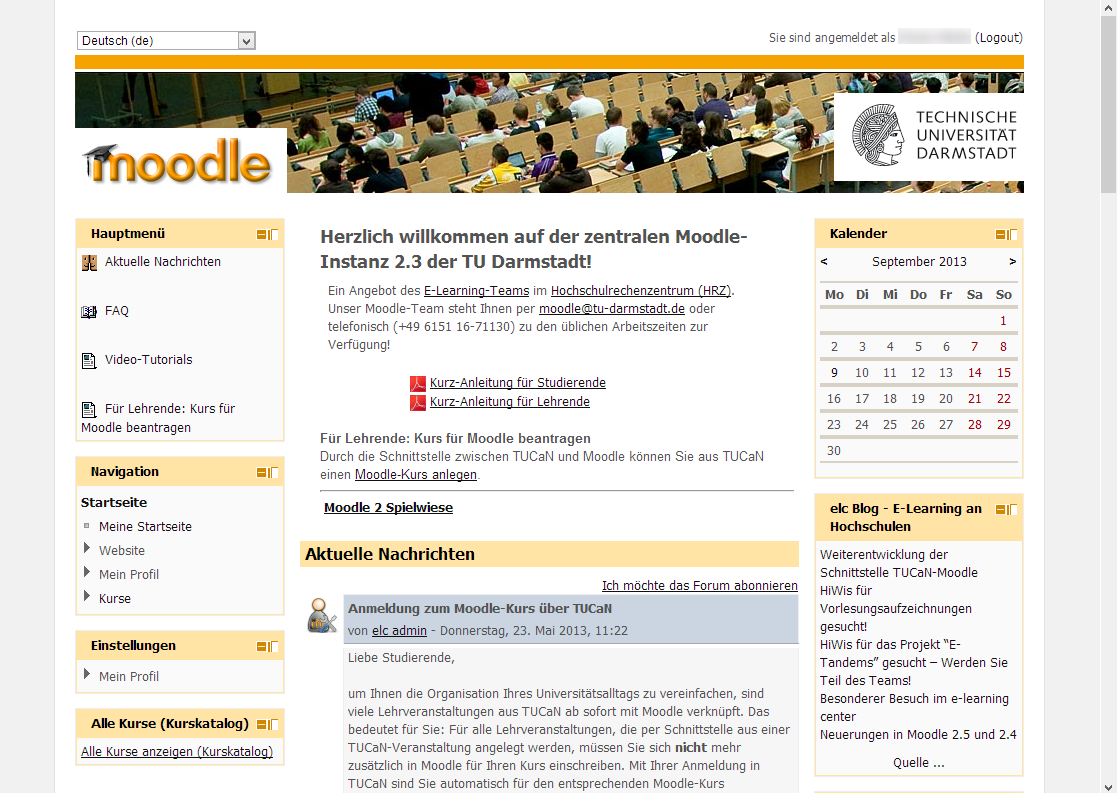
\includegraphics[
        width=0.7\textwidth,
        keepaspectratio=true,
    ]{assets/images/tud_moodle_screenshot}
    \caption{Moodle Instanz der TU Darmstadt}
    \label{fig:moodle_tud}
\end{figure}

Moodle wurde in der Programmiersprache PHP geschrieben und unterstützt die  Datenbanken werden MySQL, PostgrSQL, MSSQL und Oracle. Die Installation von weiteren Funktionalitäten ist durch von Dritten geschriebenen Erweiterungen möglich. Seit Version 2.0 können für Moodle auch Webservices installiert werden, so können auch externe Anwendungen auf interne Funktionen und Daten zugreifen.

% subsection moodle (end)

\subsection{Canvas} % (fold)
\label{sub:canvas}

Das von der Firma Instructure\footnote{\url{https://www.instructure.com/}} entwickelte \emph{Canvas} ist ein unter Open Source Lizenz gestelltes LMS. Vom Funktionsumfang ist es Moodle nicht unähnlich. Es existiert eine Verwaltung einzelner Kurse. Innerhalb dieser Kurse können in einem Forum Diskussionen geführt und Lernmieteralien hoch- und heruntergeladenen werden. Verteilung von Aufgaben, deren Benotung und ein Benachrichtigungssystem existiert ebenfalls. Canvas erlaubt auch das Einbinden von externen Diensten zum kollaborativen Lernen und Arbeiten wie Google Docs\footnote{\url{https://drive.google.com}} oder der Webkonferenz Anwendung BigBlueButton\footnote{\url{http://www.bigbluebutton.org}}.

\begin{figure}[ht]
    \centering
    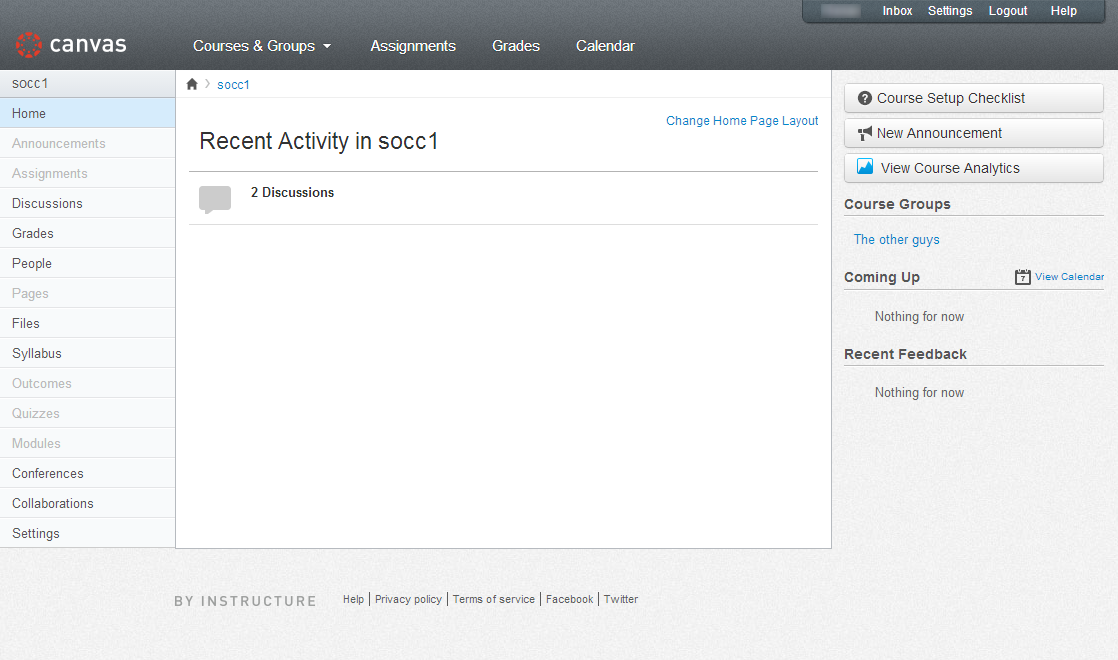
\includegraphics[
        width=0.7\textwidth,
        keepaspectratio=true,
    ]{assets/images/canvas_lms}
    \caption{Instructure Canvas}
    \label{fig:canvas_lms}
\end{figure}

Canvas wird mittels des Webframeworks \emph{Ruby on Rails}\footnote{http://rubyonrails.org/} entwickelt. Das Aussehen ist etwas moderner, als das von Moodle und es wird sehr stark auf die neuesten Webtechnologien wie HTML5 CSS3 und JQuery gesetzt. Eine Erweiterung der Funktionalität von Canvas ist durch das einbinden von Programmen möglich, die den \emph{Learning Tools Interoperability™} (LTI) Standard erfüllen. Einige solcher Programme finden sich auf der Webseite \url{https://www.edu-apps.org}. Unter anderem Programme zum Suchen und Einbinden von Youtube Videos, Wikipedia Artikeln, GitHub Gists\footnote{\url{https://gist.github.com}} und vielen weiteren.

% subsection canvas (end)

\subsection{Youtube} % (fold)
\label{sub:youtube}

Die Youtube\footnote{\url{https://www.youtube.com}} Webseite gehört wohl heute zu den beliebtesten Anlaufpunkten im Internet, wenn es um das Thema Videos geht. Monatlich nutzen über 1 Milliarde Nutzer die Seite und pro Minute werden 100 Stunden neuer Videos hochgeladen \cite{youtube2013statistics}. Doch nicht das komplette Videomaterial besteht aus Katzen, Musik oder Videos von Unfällen. Ein Teil der Benutzer die eigene Videos hochladen, wollen anderen Dinge beibringen, weil es sie schon immer interessierte oder früher selber Probleme damit hatten. Einer erklärt die Logarithmengesetze, ein anderer wie man Feuer ohne Feuerzeug macht und eine ganz andere gibt Schönheitstipps. Youtube ist also auch im E-Learning Bereich gut einsetzbar. Lehrende können eigene Videos hochladen, von anderen interessante Videos in Playlisten zusammenfassen und die Lernenden können über Kommentare Fragen zum Inhalt stellen. 

% subsection youtube (end)

\subsection{Facebook} % (fold)
\label{sub:facebook}

Das soziale Online-Netzwerk Facebook\footnote{\url{https://www.facebook.com/}} kann mit rund 699 Millionen aktiven Benutzern täglich \cite{Facebook2013} zu den aktuell beliebtesten Vertretern seiner Art bezeichnet werden. Facebook erlaubt es, wie alle sozialen Online-Netzwerke, bekannte Personen in Freundeslisten zusammen zufassen und mit ihnen private Nachrichten auszutauschen. Beiträge wie Texte, Fotos oder Videos können auf einer Art Pinnwand der \enquote{Wall} öffentlich oder nur mit Freunden geteilt werden. Benutzer mit gemeinsamen Interessen können dazu eigene Gruppen bilden und dort auf einer eigen Wall Beiträge veröffentlichen oder die anderer kommentieren. Wie in der Einleitung schon erklärt zeigt Qiyun Wang et. al. \cite{Wang2012} das sich Facebook, wenn auch mit Einschränkungen, wunderbar zur Verwaltung und Nutzung durch Lernkurse und Lerngruppen eignet. Die gleiche Erfahrung teilte Anthony Fontana \cite{Fontana2009,FacebookinEducarion2010}, der Facebook als Alternative zum bestehenden System der Bowling Green State University in Ohio, USA verwendete.

% subsection facebook (end)

\subsection{Google+} % (fold)
\label{sub:google_plus}

Google+\footnote{https://plus.google.com} ist ein 2011 von Google gestartetes soziales Online-Netzwerk. Seit Anfang 2013 ist Google+, von der Anzahl der aktiven Benutzer her gesehen, auf Platz 2 hinter Marktführer Facebook \cite{Thomas2013}. Vom Funktionsumfang sind sich beide sehr ähnlich. Auf Google+ können andere Benutzer in sogenannten \enquote{Circles} sortiert werden. Dies entspricht ungefähr den auf Facebook genutzten Freundeslisten. Jeder Benutzer hat einen eigenen \enquote{Stream} in dem er Beiträge öffentlich oder nur für ein oder mehrere Circles verfassen kann. Das Gründen von Gruppen für bestimmte Interessensbereiche ist auch in Google+ möglich und werden dort als \enquote{Communities} bezeichnet. Eines der interessantesten Funktionen von Google+ dürfte die Einführung von \enquote{Google Hangout} sein. Hier können Benutzer neben Chats auch Videokonferenzen mit bis zu zehn anderen abhalten, ohne einen externen Service wie Skype\footnote{\url{http://www.skype.com/}} zu nutzen. Diese Funktion wäre gut für den Einsatz in E-Learning nutzbar. Ein Tutor könnte so in kleiner Runde Fragestunden abhalten oder Gruppen Treffen abhalten.

% subsection google_ (end)

% section lernplattformen_und_soziale_online_netzwerke (end)

\section{Verwandte Arbeiten und Projekte} % (fold)
\label{sec:verwandte_arbeiten_und_projekte}

\todo[inline]{Verwandte Arbeiten Einleitung schreiben}

\subsection{What happens when Facebook is gone?} % (fold)
\label{sub:what_happens_when_facebook_is_gone}

Frank McCown und Michael L. Nelson beschreiben in ihrem Bericht \enquote{What happens when Facebook is gone?}\cite{McCown2009}, wie Möglichkeiten aussehen können, die unsere Daten von sozialen Online-Netzwerken (hier im speziellen Fall von Facebook) für uns und die Nachwelt archivieren können. Zum Beispiel, wenn eine Person einen großen Teil seines persönlichen Lebens auf Facebook verbringt und plötzlich stirbt. Wie sollen seine Angehörigen an nicht öffentliche Texte, Bilder, Videos heran kommen, wenn sie in der Regel keinen Zugriff auf das Benutzerkonto haben, da der Verstorbene so etwas nicht vorhersehen konnte. Oder wenn ein Benutzer mit seinen Daten in ein anderes soziales Online-Netzwerk umziehen will, sei dies bei Facebook zum damaligen Zeitpunkt nur schwer möglich.

\begin{quote}
    \enquote{It is also likely he was not prepared to die at such a young age, and much of his personal life, which lies in the digital \grqq cloud\grqq, may never be accessible to his loved ones}
    \cite[S.\,251]{McCown2009}
\end{quote}

Zum Anlegen eines solchen Archivs wurden mehrere Ansätze vorgestellt. Die einfachste Ansatz wäre die E-Mail-Benachrichtigung zu aktivieren und alle neuen Beiträge in einem E-Mail-Postfach zu sichern. So können aber nur neuen alle Beiträge erfasst werden, alte bleiben weiterhin in Facebook. Eine sehr aufwändige Möglichkeit wäre es Bildschirmfotos von den Beiträgen zu machen und diese durch ein Texterkennungsprogramm laufen zu lassen. Die dadurch erzeugten Dateien können dann in einer Datenbank gespeichert werden. Heutige Internetbrowser zusätzlich zum Anzeigen von Webseite auch der Herunterladen selbiger an. Dabei wird die HTML-Datei inklusive aller darin enthaltenen weiteren Dateien wie Bilder, Videos und CSS-Dateien gespeichert. Die so archivierte Seite hat dann im beschränkten Umfang genau das gleiche Aussehen und Verhalten wie die original Seite. Ebenfalls wäre eine Nutzung der von Facebook bereitgestellten API für Anwendungen eine Überlegung wert. 2009 war diese API noch sehr eingeschränkt. Gerade der Zugriff auf Beiträge und private Nachrichten war nicht möglich \cite[S.\,253, Table 1]{McCown2009}. Für die Implementierung eines Beispiel Programms wurde ein fünfter Ansatz gewählt. Über einen sogenannten Webcrawler oder eine Erweiterung für den Browser werden relevante Seiten automatisch heruntergeladen und in einen Archiv abgelegt. Dynamische Inhalte sollen kein Problem darstellen, da Seite erst heruntergeladen wird, wenn alle Aufrufe dynamischer Funktionen abgeschlossen ist. Die archivierten Dateien können dann mittels Datamining Techniken verarbeitet und als Atom/RSS Feed\footnote{\url{http://www.rssboard.org/rss-specification}} bereitgestellt werden. 

% subsection what_happens_when_facebook_is_gone_ (end)

\subsection{Reclaim Social} % (fold)
\label{sub:reclaim_social}

Hat sich nicht jeder schon einmal vor den Rechner gesessen um, zum Beispiel, nach einen Bild gesucht das man irgendwann auf irgendeinem der unzähligen sozialen Netzwerke hochgeladen hat, einem aber partout nicht einfallen will wo? Wann und wo habe habe ich den Beitrag geschrieben, der perfekt zu meiner aktuellen Arbeit passen würde? Solche oder ähnliche Fragen wurden sicherlich schon mehrere Millionen mal von verschiedenen Menschen in der Welt des Internets gestellt. Wer hätte in so einen Fall nicht gerne alles was man über die letzten Jahre an verschiedenen Stellen im Netz geschrieben, hochgeladen oder als für ihn wichtig markiert hat zentral gespeichert um es durchsuchen zu können? Genau diesem Thema haben sich Sascha Lobo und Felix Schwenzel angenommen und auf der Netzkonferenz re:publica\footnote{\url{http://re-publica.de/}} 2013 ihr gestartetes Projekt \enquote{Reclaim Social} \cite{Schwenzel2013} vorgestellt.

\todo[inline]{Das klingt ein wenig wie ein Werbetext ;-)}

Ziel mit diesem Projektes soziale Medien aus allen möglichen Quellen auf seinen eigenen Blog zu spiegeln und so einen zentrale Anlaufstelle für seine eigenen Inhalte schaffen. Aufbauend auf der weit verbreiteten Blogsoftware \enquote{WordPress\footnote{\url{http://wordpress.org/}}} und der dafür vorhandenen Erweiterung \enquote{FeedWordPress}\footnote{\url{http://feedwordpress.radgeek.com/}}. Diese Kombination ermöglichst alle Internetseiten, welche einen RSS Feed anbieten, in die Datenbank von WordPress zu spiegeln. Das Problem hierbei besteht darin, dass einige sehr beliebte Internetseiten solche RSS Feeds nicht anbieten (Facebook, Google+) oder eingestellt haben (\url{https://twitter.com}). Für einige solcher Seiten wurden \enquote{proxy-scripte}\cite[Tech Specs Details]{Schwenzel2013} implementiert, welche für diese einen RSS Feed emulieren. Zugleich können in den Feeds enthaltende Medien, wie Bilder und Videos(bisher nur als Referenz), heruntergeladen und in WordPress gespeichert werden. So ist es möglich alle gespiegelten Daten einfach zu durchsuchen oder nach bestimmten Kriterien zu filtern. Zusätzlich können alle Freunde, welche auch Reclaim Social einsetzen, in einen Kontaktliste eingetragen und so auch deren Inhalte eingebunden werden.

Aktuell befindet sich dieses Projekt noch im Alpha Stadium und die Installation ist relativ kompliziert. Es ist aber geplant eine eigene Erweiterung für WordPress zu schreiben \enquote{he goal is to build just one Reclaim Social-plugin for any wordpress user}\cite[How Does It Work]{Schwenzel2013}

% subsection reclaim_social (end)

% section verwandte_arbeiten_und_projekte (end)

% chapter grundlagen (end)